% !TEX root = ../../thesis.tex


\chapter{Motivations and Methodology}

\textbf{Keywords:} rapid prototyping - body design - body as an experimental variable - experimentation - 3D printing - open-source - open science


\section{Introduction} % (fold)

In chapter REF, we discussed the emergence of a novel paradigm in the robotics field in the late 80's: the embodied artificial intelligence rejects the symbolic approach and postulates that it is not possible to have intelligence without the body and the environment~\cite{pfeifer2001understanding}.
Thus an interesting evolution of the last decades is the demonstration of the importance of the morphology for sensorimotor control, cognition and development.
Exploring the interaction between body properties and cognition could lead to both a better understanding of animals’ behaviour (human being in particular) and to build robot more adapted and robust to an open environment with unpredictable interactions. In particular we can highlight the acquisition of sensorimotor tasks and the exploration of adapted bodies for natural physical and social interaction with humans.

In this context, we should not only take care of the robot body design but both introduce the morphology as an experimental variable and conduct experiments in the real world, indeed \emph{The world is its own best model} - Rodney Brooks~\cite{brooks1991intelligence}. This is especially the case of dynamic task such as the biped locomotion, t

The role of the morphology appears as a fascinating open field.
However such experiments raised two major issues researchers tried to avoid for years by using simulation. First, having a robot moving in the real world leads to problems linked to the platform robustness against mistake. An efficient experimental platform should not break itself while acting in the real world and at least, it should be easy to repair it in case of problem. Second, considering morphology as an experimental variable raised two major epistemological problems:




So exploring the morphology raises two main problem:
First, how can we modify easily and quickly the morphology of a physical robotic platform ?
Second, how can we make our work reproducible in other lab ?

In chapter Ref, we presented a review of both commercial and laboratory prototype robot platforms. The current platform are not suitable for these challenges. They do not permit the exploration of the morphology because they are not open source or the hardware is to complicated/expensive to be modified. The others are lab prototype mainly handcrafted and specifically tuned.

However, with the arrival of the "internet of things" trough low cost pro\cite{anderson}

Cependant certains changement societaux viennent boulverser le context et les habitudes. Ainsi l'emergence du monde des markers a permi l'arrivé de moyens de productions numérique low cost et efficient. L'internet des objets est maintenant possible et est en train de provoquer une révolution industrielle.
Cette revolution change le paradigm de la production comme internet a permi une ouverture du logiciel, il est maintenant possible d'avoir une ouverture du monde hardware.

Our desired is to reduce as much as possible the time required between having an idea and actual experimentation in the real world.

% Task

Also joining the new horizons of makers with the need for research in robotics can

Ainsi l'enjeux est de trouver de nouvelle methode experimentale permettant de facilement rendre le corps comme variable experimentale.

Nous proposons ici de presenter l'approche que nous avons suivi pour explorer la morpho tout en restant ouvert vers la communauté.

% Object
Nous verrons que les side effects de ces choix ont des consequences interessantes et pertinentes pour d'autres domaines scientifiques, permettant de réunir des acteurs pluridisciplianire et complémentaire dans une même communauté.

Tout en favorisant la diffusion scientifique et le bottom-up.

Along our work on building cognitive and developmental learning algorithms \cite{Oudeyer07},\cite{moulin2013exploration}, we had faced these issues and unfortunately no existing platform was available yet. Following the work we made with Acroban~\cite{Ly2010}, we designed a whole new platform called Poppy, which aims to tackle these issues. As theses issues are encountered not only in our lab but also in the robotic community, we decided right from the beginning to make the platform easily accessible to anyone. For this purpose, we designed the robot to be easy to use and to reproduce but also we distribute it freely under open source licenses (both for hardware and software).

The challenges raised by the development of such platform and its diffusion in the research community take part of the Poppy project which aims to offer an highly-hackable robotic platform.

\section{The chosen approach} % (fold)

Create robot those conception permits to easily and quickly explore morphological variants.

Create robot which can be easily reproduced in other lab.

\subsection{Exploring morphological variant with robot} % (fold)

The role of the morphology appears as a fascinating open field of research and until now not so explored. Indeed, as we saw in the chapter REF, the way to design and produce robot is a really complicated, time-consuming and costly process. To be achieved, the current robotic platforms have required dozens of engineers working for years and the raise of important founding for the production. In this context, having to change constantly the morphology to explore the variation of few parameters is not possible.

However as we discussed in chapter REF, since few years, novel techniques, especially 3D printing are revolutionizing the way we produce object. 3D printers open new horizons for the production of part, both fast and cheap. 3D printers are even able to produce parts which were either not possible or extremely costly with classical techniques.

\begin{figure}[]
    \begin{center}
        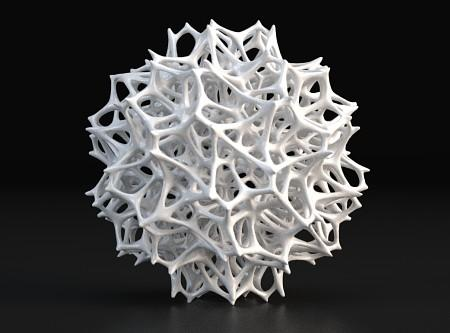
\includegraphics[width=0.8\linewidth]{complex_3Dprinted_part.jpeg}
    \end{center}
    \caption{Caption here}
    \label{fig:figure1}
\end{figure}

Propulsing the 3D printing revolution, Open hardware movement permitted the massive arrival of low cost 3D printers and multi-purpose electronic boards. So there is now affordable technologies allowing low cost production and actuation of robot.

\begin{figure}[]
    \begin{center}
        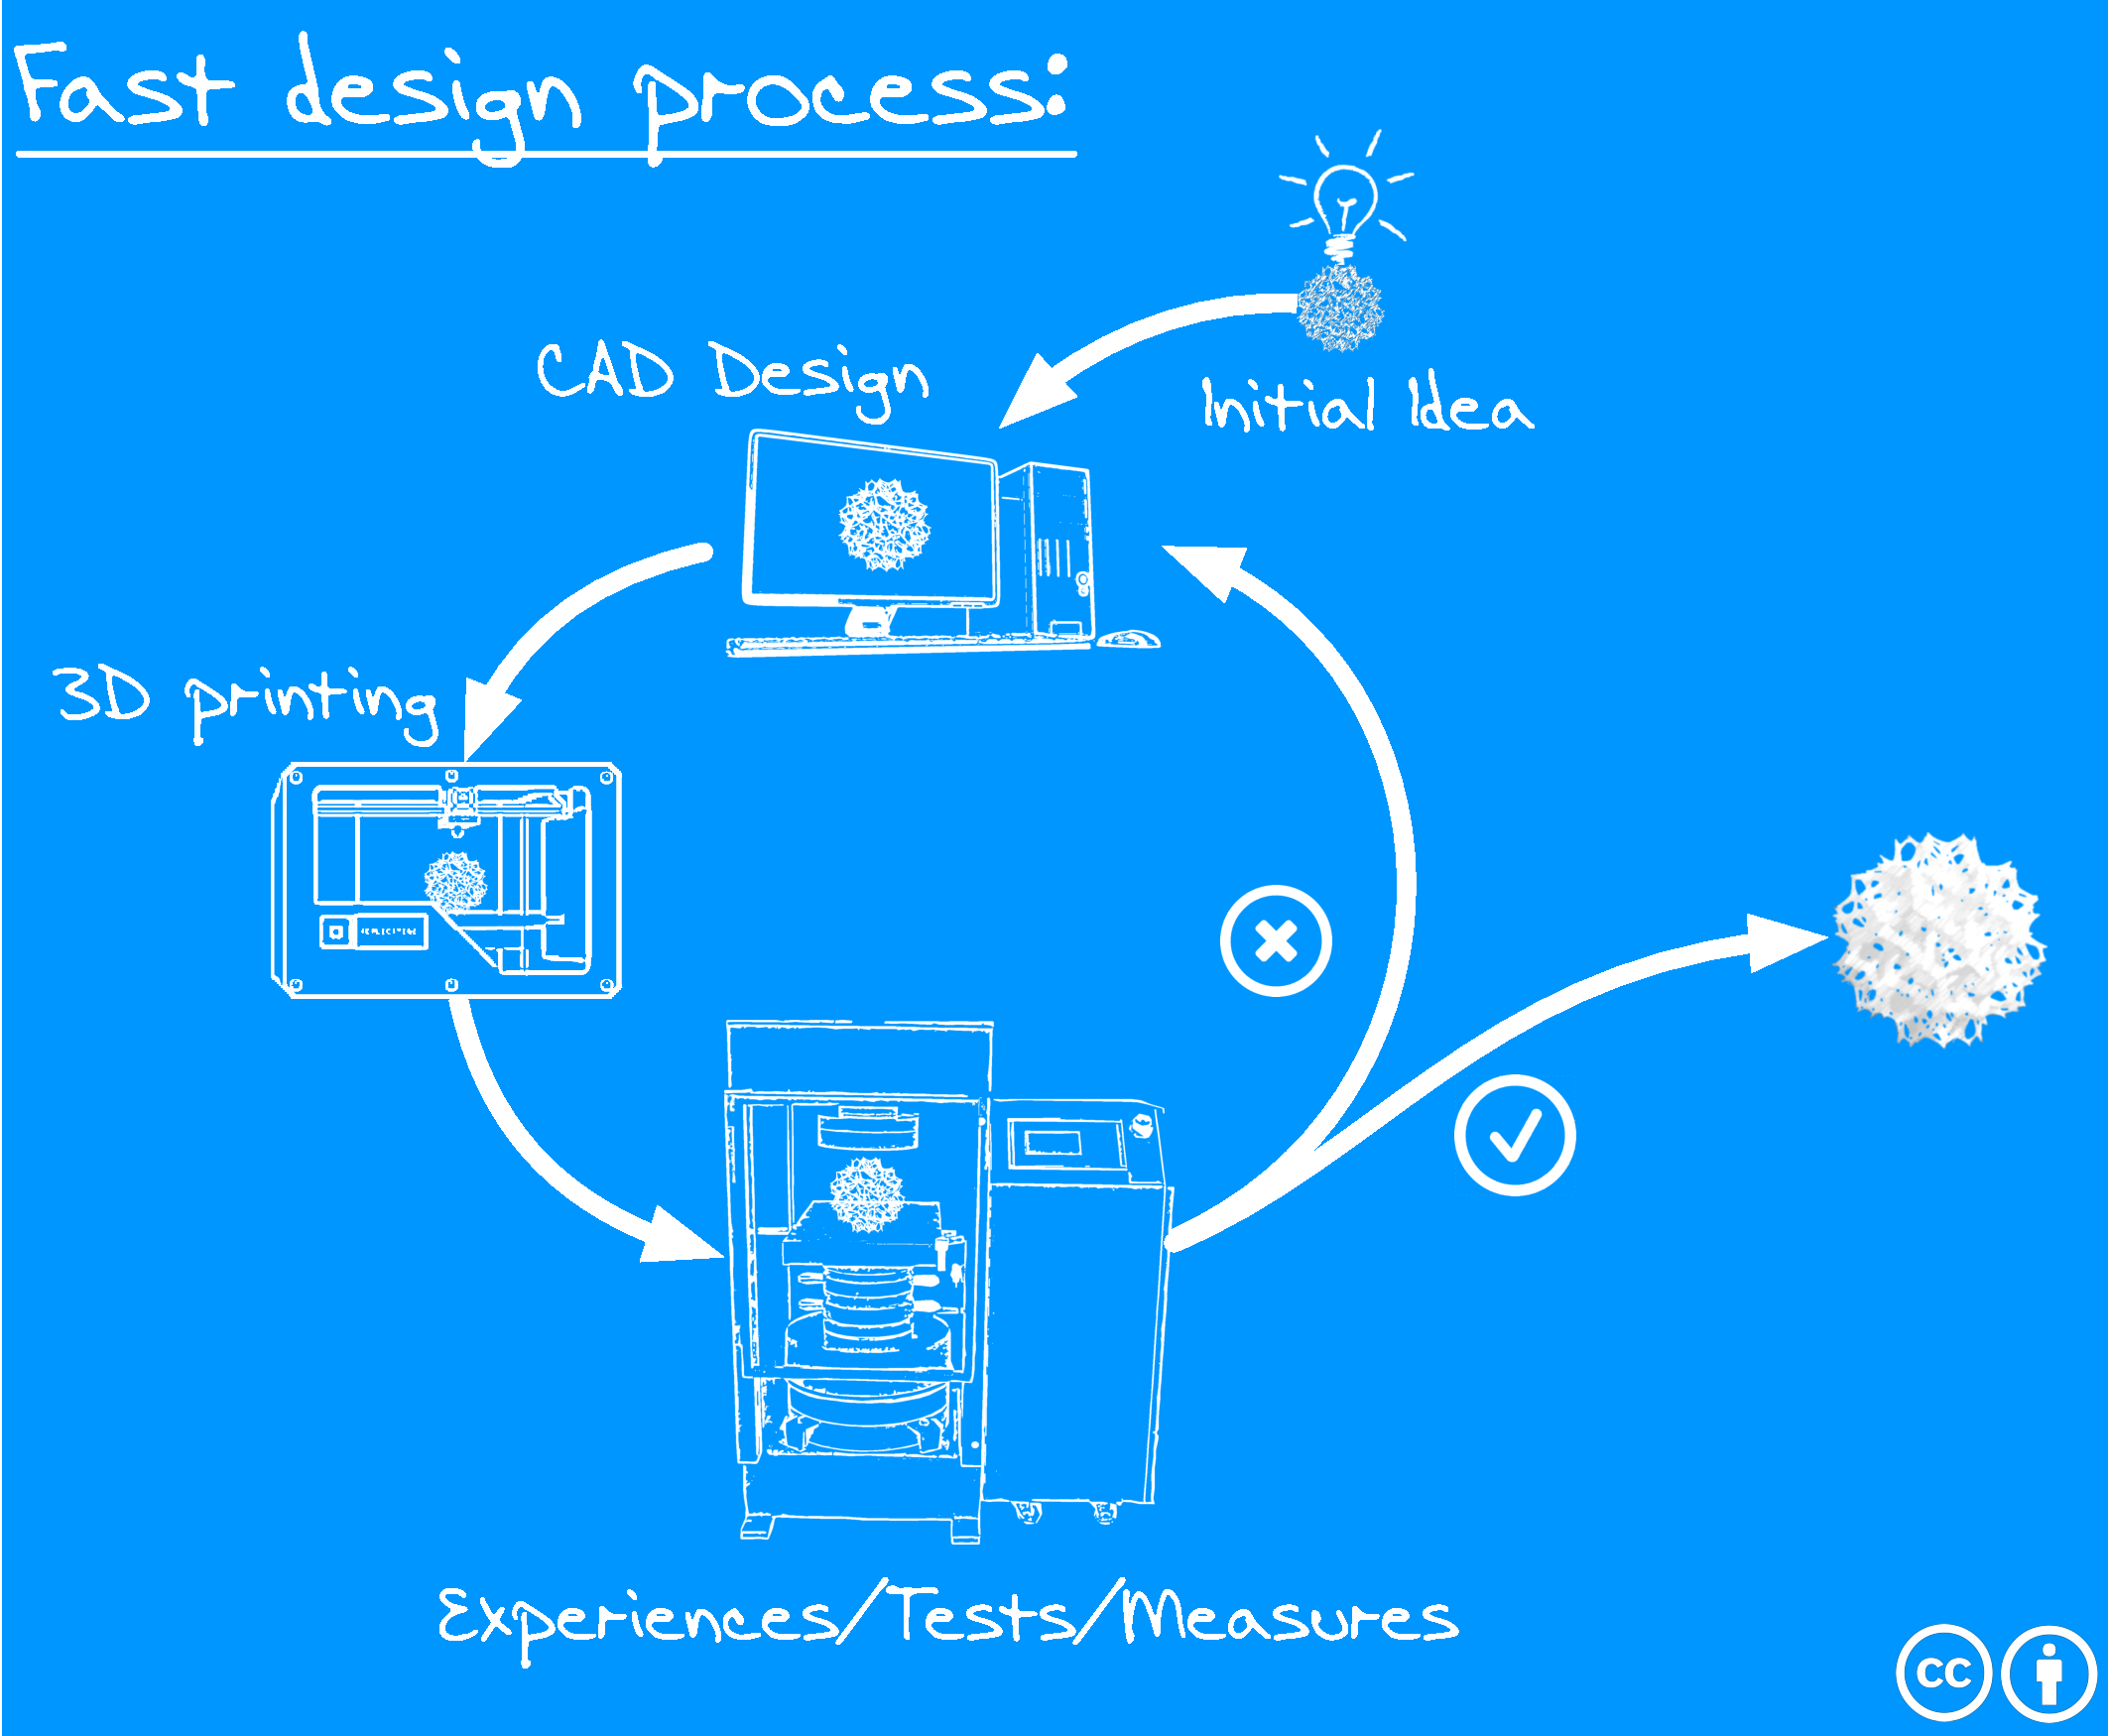
\includegraphics[width=\linewidth]{conception_iterative.pdf}
    \end{center}
    \caption{Fast conception loop}
    \label{fig:conception_loop}
\end{figure}

L'impression 3D permet de rendre le processus de design plus rapide, c'est utilisé depuis longtemps dans les centre de R\&D etc...

La difference est que maintenant, 1-on commence on garder les pièces imprimés en 3D comme finale. 2- ça devient accessible à tous, soit en achetant une imprimante soit en commandant sur internet. 3- Du coup ce qu'on propose c'est d'utiliser cette technique pour créer de la variation morphologique.


SCALABLE production tools

In this thesis we suggest to use modular 3D printed robot to explore the role of morphology.


\subsection{Make scientific work reproducible} % (fold)

In chapter REF (section REF), we discussed about very interesting robotic platform used to explore some morphological properties. However, none of these platforms can be used in other labs. They are either built using handcraft technique or costly manufacturing process. So these platforms are only used by the lab which create them and the transposition to other robot is difficult.

We think it is essential for the robotic research to make the necessary effort to make the scientific work reproducible. First, it permits an external validation of argued results. Second, it enables cumulative science which permits to accelerate the development of new technology.

\subsection{Constraints} % (fold)

Solution must be simple, reproducible, easily mountable for noobs

\section{Open} % (fold)

Logiciel et hardware sont open source. Open science et open innovation.




\section{Create an experimental platform} % (fold)

\textbf{Robustness and Safety:} The above mentioned research endeavor requires that heavy and long real-world experimentation be conducted with the robot.
This implies that the robot should be robust and safe.
It should be able to sustain experiments and fall down without easily breaking.
At the same time, one should ensure that physical interaction with the robot is safe for humans.
The approach taken is again based on morphological design, where the combination of lightweight design, compliance, and robust materials is used.
\textbf{Morphology and biped locomotion:} Studying the impact of morphology over the control and/or learning of skills requires the possibility to implement and experiment novel morphologies.
Such morphological designs were made possible with the use of 3D printing techniques.

\textbf{Social and physical human-robot interaction:} Most often, robots designed to study the role of morphology in biped locomotion do not afford rich social and physical interaction with humans: with a minimal torso and no head \cite{collins2001three}\cite{niiyama2010athlete}.
Poppy was designed to afford such full-body physical interaction (we will illustrate this with the possibility to guide him physically in biped locomotion), as well as to afford social interaction, with a head and gestural apparatus that can be programmed for communicative or affective expression.

\textbf{Full-body compliance:} Important aspects of adaptation to physical obstacles or to humans require humanoid robots to be full-body compliant.
This includes both the ability to absorb external shocks due to the passive compliance of the mechanical structure (bendable materials and springs), but also the ability to actively and dynamically control the compliance of motors, which may be either controlled in position with compliance, or directly in torque (thanks to the use of adequate recent servomotor technologies).



\textbf{Breakable, repairable:} Even if breaking should be made unusual, real-world experimentation should be expected to break the robot at regular intervals.
This should not become a problem for conducting research.
Breaking should not be costly and the robot should be easily repairable.
This is achieved thanks to 3D printing techniques, affordable off-the-shelf components, and optimized mounting design.

\textbf{Precision, stationarity:} Experiments should be repeatable, implying that the robot properties should be stationary.

\textbf{Transportable outside the lab:} To allow for experiments in natural environments, possibly involving interaction with non-technical humans, the robot should be transportable outside the laboratory.

\textbf{Easy and fast to duplicate:} Such a reuse of the robotic platform requires that it is easy and fast to duplicate.
The approach taken is to only use off-the-shelf components (motors and electronics) and limbs which can be printed with regular 3D printing services.
The Poppy humanoid platform takes two days to assemble by one user, and was already reproduced twice, including by another laboratory\footnote{Laboratoire de la Perception et de l'Action (J.Droulez), Collège de France, Paris, France\label{LPPA}}.

\textbf{Affordable:} A mid-term goal of this project is to open the hardware and software platform to the academic community (under an open-source mode), to allow other research laboratories to use it as an experimental platform.
A key aspect for such an open dissemination is to keep the cost of the robot relatively low.
The overall materials needed to build a Poppy robot cost around 7500 euros including 4700 euros for actuators, 1600 euros for of the shell mechanical and electronic components and 1200 euros for 3D printed mechanical parts.

% \end{description}

The Poppy platform presented in this article was designed to target these design goals within the context of biped locomotion.
We focus here on the presentation of the design of specific morphological parts: the hip, the thigh, the limb mesh and the knee.





\section{Developping experimental tools}

In this context, we need to find new design methodology allowing to easily explore the role of morphology and we need to find workflow to share scientific contributions with the community.

\subsection{The needs}
hardware platform keyword: robust, flexible, safety, breakable, repairable, stationnarity, affordable, Easy and fast to duplicate, modular, easy to set up.


\section{Limitations} % (fold)

On doit faire des compromis et se résoudre à ne pas faire une solution qui  nous paraissent interessantes car elle poserait problème à la diffusion.
C'est chiant mais c'est la vie pour faire de la science cumulative.
Il faut se limiter.


\section{Conclusion} % (fold)

FabLab approach: We use 3D printing, simple design, simple to use library, open source and creative commons licence.

Diffusion Open source with git repository

We find a really quick and cheap way to conceive Poppy.

Based on this work, we will be able both to explore morphology and distribute our works.

These needs share a common thread: the need of an easy to get/reproduce hardware platform.

We want to have flexible platform allowing to easily perform scientific experiments.
We do not want to spend more time on debug than doing actual experiments and then we want to be able to share our research in order to have a scientific impact.



